\documentclass[12pt]{article}

\usepackage{times}
\usepackage{textcomp}
\usepackage{listings}
\usepackage{fullpage}
\usepackage{color}
\usepackage{hyperref} 
\usepackage{pst-tree} 
\usepackage{verbatim} 
\usepackage{graphicx}
\usepackage{amsmath,amsfonts,amssymb,amsthm}
\graphicspath{ {./}}
\usepackage{courier}


\def\part#1{\item[\bf #1)]}
\renewcommand{\thesubsection}{Question \arabic{subsection}}
\lstset{language=C, keywordstyle={\bfseries \color{red}}, basicstyle=\footnotesize\ttfamily}

\author{Clement Tsang}

\begin{document}

\begin{center}
    \Large\textbf{CS 241, Lecture 16 - Type Checking and Code Generation}
\end{center}

\section{Types (cont.)}
\begin{itemize}
    \item ``The beginning of the end.'' - Carmen Bruni
    \item We note that WLP4... doesn't have booleans.  How can we do loops and ifs then?  Well, make sure for the grammar:
    \begin{lstlisting}[mathescape, numbers=none, breaklines=true]
    while (T) {S}
    if (T) {S1} else {S2}
    \end{lstlisting}
    \item Make $T$ a boolean test of type ``\lstinline[mathescape]{expr comp expr}''.
    \item The inference rules, again: \\\\
    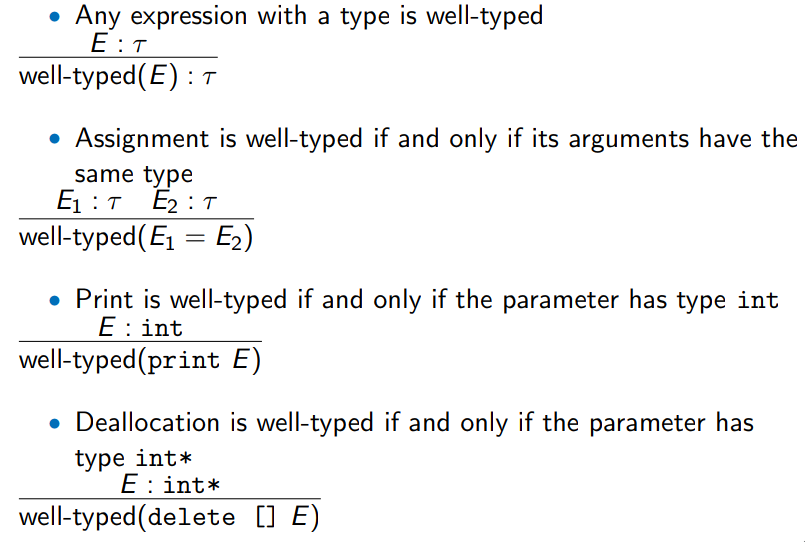
\includegraphics[scale=0.4]{inference1.png}\\
    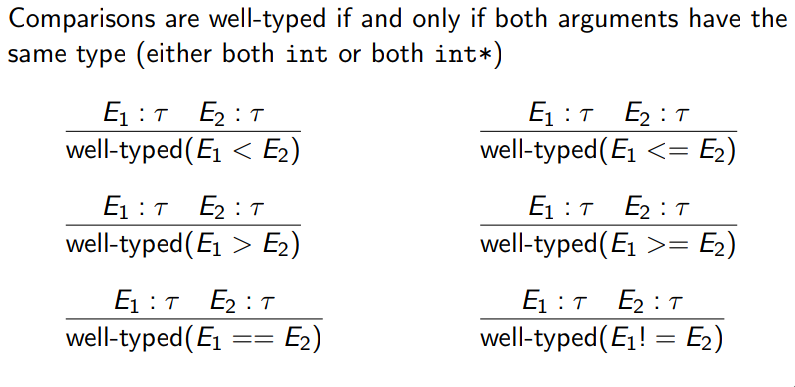
\includegraphics[scale=0.4]{inference2.png}\\
    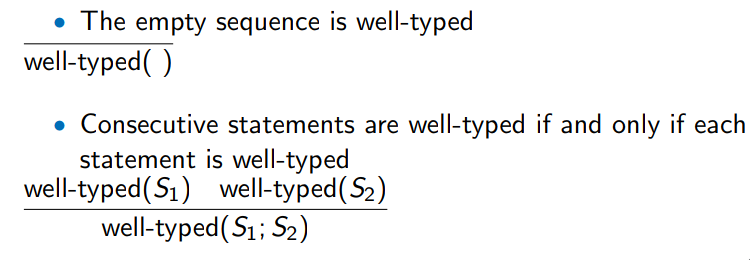
\includegraphics[scale=0.4]{inference3.png}\\
    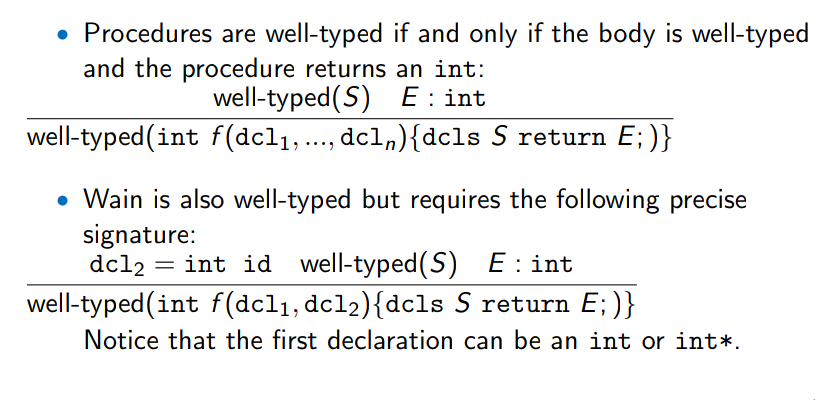
\includegraphics[scale=0.4]{inference4.png}\\
    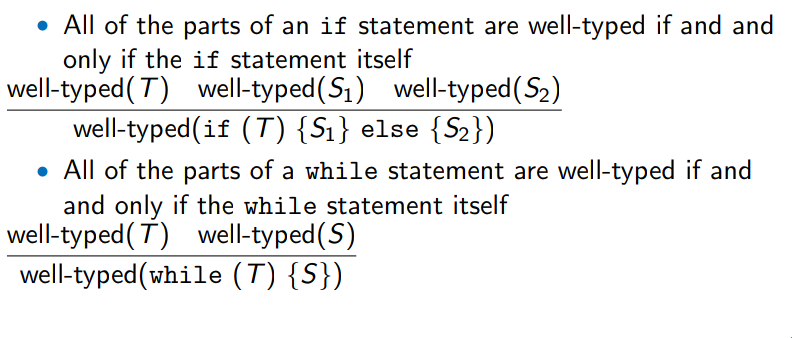
\includegraphics[scale=0.4]{inference5.png}
    \item Note for WAIN, we allow the first argument to be an int or int pointer, as we will always need the second arg to be an int (size of array in mips.array, int in mips.twoints)
    \item We call anything that is a storage location an \emph{lvalue}.  
    \item For us, lvalues are any of variable names, dereferenced pointers, or any parenthical combination of these.  NOT integers.  
    \item This is forced by the WLP4 grammar so we don't really need to manually check this!
\end{itemize}

\section{Code Generation}
\begin{itemize}
    \item We wrote code that translates WLP4 $\rightarrow$ to a grammar, and we have code that translates MIPS $\rightarrow$ binary.  So we need to fill the missing link - grammar to MIPS.
    \item We need to make sure our WLP4 and MIPS code do the same thing!  This is the most important!
    \item We also want it to be somewhat efficient - both by compile time and code itself, the latter of with we will measure this by number of lines.
    \item Now, given the following code:
    \begin{lstlisting}[mathescape, numbers=none, breaklines=true]
    int wain(int a, int b) {
        return a;
    }
    \end{lstlisting}
    what is the MIPS command?  Well:
    \begin{lstlisting}[mathescape, numbers=none, breaklines=true]
    add $\$$3, $\$$1, $\$$0
    jr $\$$31
    \end{lstlisting}
    \item But there's a \emph{slight} problem - if we wanted to return b instead, then the \emph{parse tree} of both functions would be identical!
    \item Luckily, we have a symbol table!  We will augment it to also include where each symbol is stored:\\\\
        \begin{tabular}{|c|c|c|}
            \hline
            Symbol & Type & Location \\
            \hline
            a & int & $\$1$ \\
            b & int & $\$2$ \\
            \hline
        \end{tabular}\\
    \item But... if we keep storing variables and parameters in registers, we \emph{will} run out of registers - especially recursive code!  Therefore, we're back to our old friend, the \textbf{stack}.
    \item So, our old code now for a basic wain program becomes (note I got lazy and used ``s'' instead of ``\$''):
    \begin{lstlisting}[mathescape, numbers=none, breaklines=true]
    sw s1, -4(s30)
    sw s2, -8(s30)
    lis s4
    .word 4
    sub s30, s30, s4
    sub s30, s30, s4
    lw s3, 4(s30)
    add s30, s30, s4
    add s30, s30, s4
    jr s31
    \end{lstlisting}
    \item Note by convention, $\$4$ contains the integer 4. 
    \item Also, we will now instead make the symbol table store the \emph{offset} from the stack pointer:\\\\
        \begin{tabular}{|c|c|c|}
            \hline
            Symbol & Type & Offset from $\$30$ \\
            \hline
            a & int & 4 \\
            b & int & 0 \\
            \hline
        \end{tabular}\\
    \item Variables also have to go on the stack, but we don't know what the offsets will be until we process all the variables and parameters... consider the following code and accompanying MIPS program:
    \begin{lstlisting}[mathescape, numbers=none, breaklines=true]
    int wain (int a, int b) {
        int c = 0;
        return a;
    }
    \end{lstlisting}
    \begin{lstlisting}[mathescape, numbers=none, breaklines=true]
    sw s1, -4(s30)
    sw s2, -8(s30)
    lis s4
    .word 4
    sub s30, s30, s4
    sub s30, s30, s4
    sub s30, s30, s4  ; For int c
    sw s0, 0(s30)     ; c = 0
    lw s3, 8(s30)     ; 8 from the symbol table
    add s30, s30, s4 
    add s30, s30, s4
    add s30, s30, s4  ; We could probably speed this part up
    jr s31
    \end{lstlisting}
    \item But this isn't enough... what if we have more variables?  What do we do?  Change all our offsets every time?
    \item Remember \$30 represents the \emph{top} of the stack - and \$29 represents the \emph{bottom} of the stack!  We will use \$29 to calculate our offsets, as no matter how far we move the top of the stack, the offsets from \$29 will remain unchanged!
\end{itemize}


\end{document}

